\documentclass[a4paper]{article}

%use the english line for english reports
%usepackage[english]{babel}
\usepackage[portuguese]{babel}
\usepackage[utf8]{inputenc}
\usepackage{indentfirst}
\usepackage{graphicx}
\usepackage{verbatim}


\begin{document}

\setlength{\textwidth}{16cm}
\setlength{\textheight}{22cm}

\title{\Huge\textbf{Trench}\linebreak\linebreak\linebreak
\Large\textbf{Relatório Intercalar}\linebreak\linebreak
\linebreak\linebreak

\includegraphics[scale=0.1]{feup-logo.png}\linebreak\linebreak
\linebreak\linebreak
\Large{Mestrado Integrado em Engenharia Informática e Computação} \linebreak\linebreak
\Large{Programação em Lógica}\linebreak
}

\author{\textbf{Grupo xx:}\\
Kevin Amorim - 201207231 \\
Luís Magalhães - 201207224 \\
\linebreak\linebreak \\
 \\ Faculdade de Engenharia da Universidade do Porto \\ Rua Roberto Frias, s\/n, 4200-465 Porto, Portugal \linebreak\linebreak\linebreak
\linebreak\linebreak\vspace{1cm}}

\maketitle
\thispagestyle{empty}

%************************************************************************************************
%************************************************************************************************

\newpage

%Todas as figuras devem ser referidas no texto. %\ref{fig:codigoFigura}
%
%%Exemplo de código para inserção de figuras
%%\begin{figure}[h!]
%%\begin{center}
%%escolher entre uma das seguintes três linhas:
%%\includegraphics[height=20cm,width=15cm]{path relativo da imagem}
%%\includegraphics[scale=0.5]{path relativo da imagem}
%%\includegraphics{path relativo da imagem}
%%\caption{legenda da figura}
%%\label{fig:codigoFigura}
%%\end{center}
%%\end{figure}
%
%
%\textit{Para escrever em itálico}
%\textbf{Para escrever em negrito}
%Para escrever em letra normal
%``Para escrever texto entre aspas''
%
%Para fazer parágrafo, deixar uma linha em branco.
%
%Como fazer bullet points:
%\begin{itemize}
	%\item Item1
	%\item Item2
%\end{itemize}
%
%Como enumerar itens:
%\begin{enumerate}
	%\item Item 1
	%\item Item 2
%\end{enumerate}
%
%\begin{quote}``Isto é uma citação''\end{quote}


%%%%%%%%%%%%%%%%%%%%%%%%%%
\section{O Jogo TRENCH}

\begin{figure}[h!]
\begin{center}
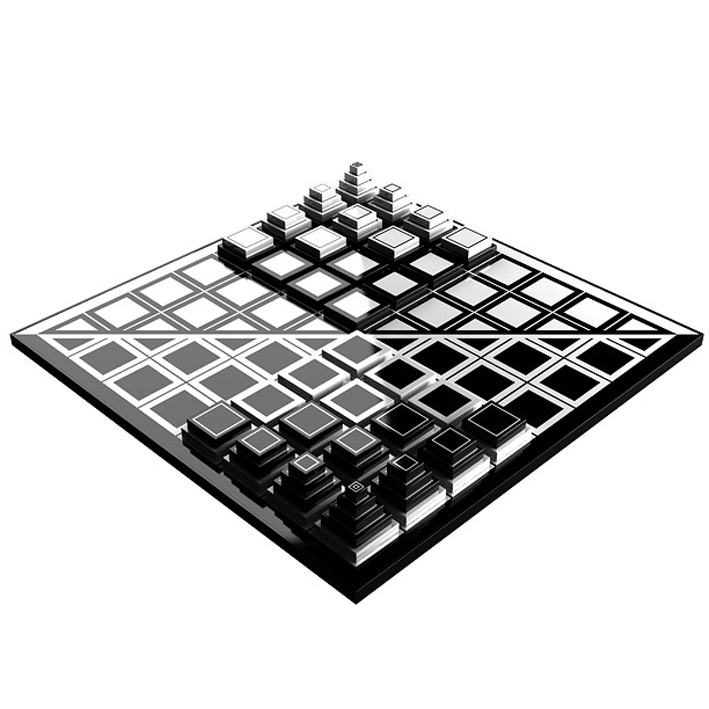
\includegraphics[scale=0.3]{img/game-cover.jpg}
\label{fig:0}
\end{center}
\end{figure}

Trench é um jogo de tabuleiro criado em Portugal por Rui Alípio Monteiro, em 2013. Este é um jogo para 2 jogadores baseado na guerra de trincheiras da 1ª Guerra Mundial. 

Os algoritmos aplicados no jogos seguem os princípios referidos no livro "The Art of the War", de Sun Tzu. A disposição das peças do jogo em losango é inspirada na formação em diamante, originária no exército romano.

\subsection{Objetivo do Jogo}

O objetivo do jogo é capturar todas as peças inimigas. No entanto, nem sempre é possível que tal aconteça (pelas limitações das peças e do tabuleiro), pelo que a vitória ou a derrota regem-se por um sistema de pontuação, explicado em baixo.

\subsection{Início do Jogo}

O jogador que possuir as peças de cor preta inicia o jogo. Cada jogador tem direito a uma jogada por turn. O jogo termina ao fim de 25 jogadas se nenhuma peça for capturada nesse intervalo.

\newpage

\subsection{Tabuleiro de Jogo}

O tabuleiro representa o campo de batalha, com as respetivas trincheiras.
O tabuleiro de jogo tem uma forma em diamante, dividido por uma linha diagonal, que representa a linha das trincheiras (Cada metade do tabuleiro tem uma cor predominante: preto para um jogador, branco para o outro).
O tabuleiro é constítuido por 64 casas (8x8), divididas em dois territórios opostos.

\begin{figure}[h!]
\begin{center}
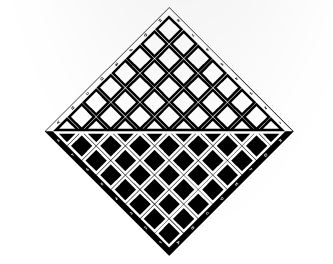
\includegraphics[scale=0.5]{img/board.jpg}
\caption{Tabuleiro de jogo 8x8}
\label{fig:1}
\end{center}
\end{figure}


\subsection{Peças do Jogo}

As peças do jogo são as apresentadas na seguinte tabela:

\begin{figure}[h!]
\begin{center}
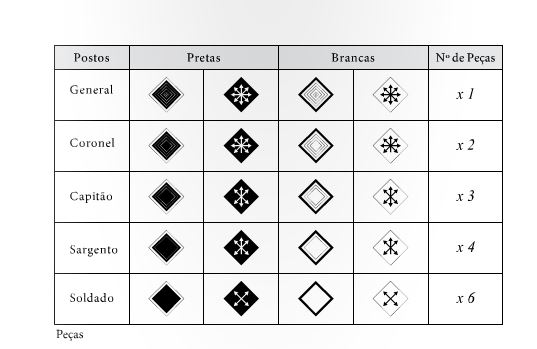
\includegraphics[scale=0.8]{img/pieces.jpg}
\caption{Tabel das peças do jogo}
\label{fig:2}
\end{center}
\end{figure}

 \newpage

Estas possuem uma forma em losango, inspirada nas estrelas usadas pelos soldados em batalha. Estas simbolizam a hierarquia militar em pirâmide.

\begin{figure}[h!]
\begin{center}
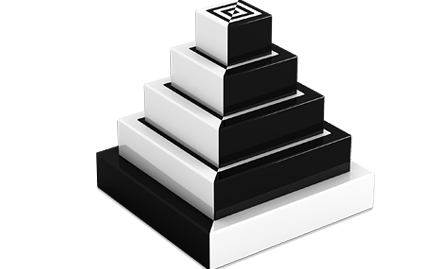
\includegraphics[scale=0.5]{img/piece.png}
\caption{Peça do jogo Trench}
\label{fig:3}
\end{center}
\end{figure}

As peças seguem a seguinte hierarquia (estando no topo o de mais alto nível):

\begin{enumerate}
	\item General
	\item Coronel
	\item Capitão
	\item Sargento
	\item Soldado
\end{enumerate}s


%%%%%%%%%%%%%%%%%%%%%%%%%%
\section{Representação do Estado do Jogo}

Descrever a forma de representação do estado do tabuleiro (tipicamente uma lista de listas), com exemplificação em Prolog de posições iniciais do jogo, posições intermédias e finais, acompanhadas de imagens ilustrativas.


%%%%%%%%%%%%%%%%%%%%%%%%%%
\section{Visualização do Tabuleiro}

Descrever a forma de visualização do tabuleiro em modo de texto e o(s) predicado(s) Prolog construídos para o efeito.
Deve ser incluída pelo menos uma imagem correspondente ao output produzido pelo predicado de visualização.


%%%%%%%%%%%%%%%%%%%%%%%%%%
\section{Movimentos}

Elencar os movimentos (tipos de jogadas) possíveis e definir os cabeçalhos dos predicados que serão utilizados (ainda não precisam de estar implementados).


\end{document}
